%! TEX root = main.tex

\graphicspath{{00_Images/03_chapter/}}

\chapter{The Acoustic Domain}
\label{ch:acoustical_twoport}

The third domain in the transduction chain is the acoustical domain. Once the tools for mapping mechanical quantities to electrical ones are in place, extending the analogy to acoustics requires only identifying the correct power variables and deriving the constitutive relations for the three fundamental acoustic elements: mass, resistance, and compliance.

\section{Acoustic Variables and Fundamental Elements}
\label{sc:31}

In the acoustical domain the two power variables are acoustic pressure \(P\) (in pascal, \(\si{\pascal} = \si{\newton\per\meter\squared}\)) and volume velocity \(U\) (in cubic meters per second, \(\si{\cubic\meter\per\second}\)). Volume velocity is defined as:
\[
U = u \cdot S_D
\]
where \(u\) is the particle velocity and \(S_D\) is the cross-sectional area through which sound propagates, for instance the diaphragm area. The instantaneous acoustic power flowing through a cross-section is:
\[
P_A = P \cdot U
\]
This is the direct acoustic counterpart of \(P_E = v i\) in the electrical domain and of \(P_M = F u\) in the mechanical domain. The acoustic impedance of a one-port element is defined as:
\[
Z_A = \frac{P}{U} \quad \left[\frac{\si{\pascal}}{\si{\cubic\meter\per\second}} = \frac{\si{\newton\second}}{\si{\meter\tothe{5}}}\right]
\]
The specific acoustic impedance, which refers to particle velocity rather than volume velocity, is related to \(Z_A\) by \(Z_s = Z_A \cdot S\) and is measured in Rayls (\(\si{\pascal\second\per\meter}\)). For a plane wave in free air, the specific acoustic impedance equals the characteristic impedance of the medium, \(Z_0 = \rho_0 c \approx \SI{407}{\text{Rayl}}\).

\subsection{Acoustic Mass}
\label{ssc:311}

The acoustic mass \(M_A\) (in \(\si{\kilo\gram\per\meter\tothe{4}}\)) models the inertia of an air volume set in motion. It arises whenever a column of air is accelerated, for example inside a tube, a port, or the neck of a Helmholtz resonator. Its relation to the mechanical mass is:
\[
M_A = \frac{M_M}{S^2}
\]
because dividing the mechanical equation \(F = M_M du/dt\) by \(S^2\) and using \(P = F/S\), \(U = u S\) gives the acoustic constitutive relation:
\[
P = M_A \frac{dU}{dt}
\]
This has the same form as \(v = L di/dt\) for an inductor, so under the impedance analogy (\(P \leftrightarrow v\), \(U \leftrightarrow i\)), the acoustic mass corresponds to an inductor of value \(L_E = M_A\). Its acoustic impedance in the sinusoidal regime is \(Z_{M_A} = j\omega M_A\), which increases linearly with frequency and dominates the acoustic response at high frequencies.
Under the admittance analogy (\(P \leftrightarrow i\), \(U \leftrightarrow v\)), the same equation \(P = M_A dU/dt\) maps to \(i = C_E dv/dt\), so the acoustic mass corresponds to a capacitor of value \(C_E = M_A\). In practical terms, a large enclosed air volume behind a loudspeaker diaphragm contributes an acoustic mass load that appears, in the equivalent circuit, as either an inductor or a capacitor depending on the chosen analogy.

\begin{figure}[!htb]
    \centering
    \subfloat[Modeled as an inductor under the impedance analogy (\(P \leftrightarrow v\), \(U \leftrightarrow i\))]{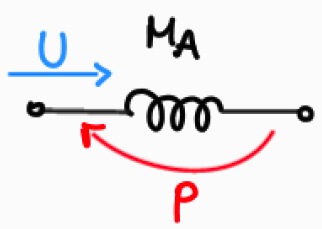
\includegraphics[width=0.3\linewidth]{acoustic_mass_impedance.png}}
    \hspace{1cm}
    \subfloat[Modeled as a capacitor under the admittance analogy (\(P \leftrightarrow i\), \(U \leftrightarrow v\))]{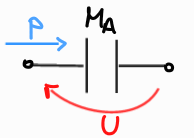
\includegraphics[width=0.3\linewidth]{acoustic_mass_admittance.png}}
    \caption{Both model of the acoustic mass}
\end{figure}

\subsection{Acoustic Resistance}
\label{ssc:312}

The acoustic resistance \(R_A\) (in \( \si{\newton\second\per\meter\tothe{5}} \)) models the power dissipated by viscous friction as air flows through a constriction such as a porous material, a narrow tube, or the perforations of a diaphragm. Starting from the mechanical damper relation \(F = R_M u\) and dividing by \(S^2\):
\[
P = R_A U, \qquad R_A = \frac{R_M}{S^2}
\]
This maps directly to \(v = R i\) in the electrical domain: under both the impedance and admittance analogies, the acoustic resistance corresponds to a resistor (or conductance, depending on the convention). Its acoustic impedance is purely real, \(Z_{R_A} = R_A\), independent of frequency, and mean power is dissipated at the rate \(\overline{P_A} = R_A U_\mathrm{RMS}^2\).
A practical acoustic resistance arises, for example, in a rectangular block of height \(2b\), width \(w\), and depth \(t\), drilled with cylindrical holes of radius \(a\). Each hole presents both a resistive and a mass contribution, with the resistance arising from viscosity and the mass from the inertia of the air slug inside the hole. Under the impedance analogy these two contributions appear in series, giving for each hole:
\[
Z_A = R_A + j\omega M_A
\]
with analytical expressions:
\[
R_A = \frac{1}{\pi a^2}\sqrt{\frac{2\omega\mu}{\rho_0}} \cdot \left[\frac{t}{a} + 2\left(1 - \frac{\pi a^2}{b^2}\right)\right],
\qquad
M_A = \frac{\rho_0}{\pi a^2}\left[t + 17a\left(1 - \frac{a}{b}\right)\right]
\]
where \(\mu\) is the dynamic viscosity of air and \(\rho_0\) is the air density. Such structures appear in loudspeaker cabinet design, microphone grilles, and acoustic absorption panels.

\subsection{Acoustic Compliance}
\label{ssc:313}

The acoustic compliance \(C_A\) (in \(\si{\meter\tothe{5}\per\newton}\)) models the elastic behavior of an enclosed volume of air. When a piston of area \(S\) compresses a cavity of volume \(V_0\), the restoring pressure is proportional to the fractional volume change, exactly as a spring restores a displaced mass. Starting from Hooke's law \(x = C_M F\) and converting to acoustic variables:
\[
U = C_A \frac{dP}{dt}, \qquad C_A = C_M S^2
\]
This has the same form as \(i = C dv/dt\) for a capacitor. Under the impedance analogy (\(P \leftrightarrow v\), \(U \leftrightarrow i\)), the acoustic compliance therefore corresponds to a capacitor of value \(C_E = C_A\). Its acoustic impedance is \(Z_{C_A} = 1/(j\omega C_A)\), which dominates the response at low frequencies. Under the admittance analogy (\(P \leftrightarrow i\), \(U \leftrightarrow v\)), differentiating the relation gives \(P = (1/C_A)\int U dt\), which maps to \(v = L di/dt\) for an inductor, so the acoustic compliance corresponds to an inductor.

\begin{figure}[!htb]
    \centering
    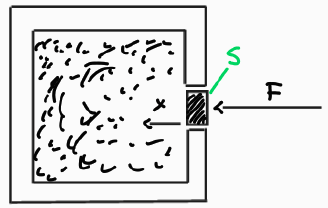
\includegraphics[width=0.5\linewidth]{acoustic_compliance_box.png}
    \caption{Acoustic compliance: a sealed box of volume \(V_0\) behind the diaphragm behaves as a spring. The equivalent acoustic compliance is \(C_A = V_0/(\rho_0 c^2)\) for an adiabatic process}
\end{figure}

For an adiabatic compression of an ideal gas in a rigid enclosure of volume \(V_0\), the acoustic compliance is:
\[
C_A = \frac{V_0}{\gamma P_0}
\]
where \(\gamma \approx 1.4\) is the ratio of specific heats and \(P_0 \approx \SI{101325}{\pascal}\) is the ambient pressure. A larger box is more compliant (softer spring), so its resonance with an acoustic mass occurs at a lower frequency. This is the physical basis for the dependence of a loudspeaker's bass response on enclosure volume.

\paragraph{Summary of acoustic element analogies} Under the impedance analogy, the acoustic mass maps to an inductor, the acoustic compliance maps to a capacitor, and the acoustic resistance maps to a resistor, with \(Z_A = P/U\) playing the role of electrical impedance. Under the admittance analogy, mass and compliance exchange their circuit roles (capacitor and inductor respectively), while resistance maps to a conductance. In both cases, acoustic power is conserved in the lossless elements and dissipated only in the acoustic resistance.
